\documentclass[docmute]{article}

\usepackage[margin=1in]{geometry}


% AMS packages for enhanced math typesetting and symbols:
\usepackage{amsmath}  % Provides enhanced math features like align, gather, etc.
\usepackage{amssymb}  % Provides additional math symbols
\usepackage{amsthm}   % Enables theorem-like environments

\usepackage{graphicx} % Provides commands for including and managing external graphics (e.g., figures, images)

% Package for customizing list environments:
\usepackage{enumitem} % Allows control over layout of lists (itemize, enumerate, etc.)

% Full-page layout package:
\usepackage{fullpage} % Uses more of the page area by reducing margins

% TikZ package for drawing graphics:
\usepackage{tikz}     % Used for creating high-quality diagrams and figures

% Microtype package for typographical enhancements:
\usepackage{microtype} % Improves justification, kerning, and overall appearance

% Package for typesetting polynomials:
\usepackage{polynom}  % Provides commands for polynomial long division and related tasks

% Package for controlling figure placement:
\usepackage{placeins} % Provides the \FloatBarrier command to control floating environments

% Forest package for drawing trees:
\usepackage{forest}   % Simplifies the creation of tree diagrams

% Package to allow one LaTeX file to input another:
\usepackage{docmute}  % Allows this file to be included in another document without reloading the preamble

% Load additional TikZ libraries:
\usetikzlibrary{trees} % Provides additional tree-specific commands for TikZ

% Define theorem-like environments using amsthm:
\newtheorem{corollary}{Corollary} % Defines a new "corollary" environment
\newtheorem{lemma}{Lemma}         % Defines a new "lemma" environment

\input{watermark/watermark.tex}

\title{Graphs}
\author{Tomasz Brengos}
\date{}

\begin{document}
\maketitle


\section{Formal definition}
% HEHHE
A graph is a pair \(G=(V,E)\) where \(V\) is a finite non-empty set (called the set of  \emph{vertices}) 
and \(E\) is a set (called the set of \emph{edges}), where \(E \subseteq \binom{V}{2}\) (all two-element subsets of \(V\)).
\medskip

Notation:\medskip

If G=\((V,E)\), then  \(V =: V(G)\) and \(E =: E(G)\).
\medskip

If \(\{u,v\} \in E\), then we write \(uv \in E\) (\(vu=uv\), as edges are unordered)
\medskip

If \(u,v \in V(G)\) such that \(uv \in E(G)\), then we say that \(u\) and \(v\) are \emph{connected} by an edge in \(G\)
\medskip

\subsection*{Example}
Let \(G = (V,E)\) where \(V = \{a,b,c\}\) and \(E = \{\{a,b\}, \{a,c\}\}\).
This can be visualized as:
\begin{center}
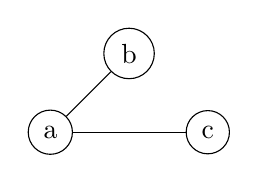
\begin{tikzpicture}
  \node[draw, circle] (a) at (0,0) {a};
  \node[draw, circle] (b) at (1,1) {b};
  \node[draw, circle] (c) at (2,0) {c};
  \draw (a) -- (b);
  \draw (a) -- (c);
\end{tikzpicture}
\end{center}

\section{Basic Concepts and Terminology}

\subsection*{Simple Graphs}
A graph is called \textbf{simple} if it is non-oriented (undirected), has no loops (edges from a vertex to itself), and is not a multigraph (has at most one edge between any pair of vertices). The definition provided in Section 1 refers to simple graphs.

\subsection*{Isomorphism}
We say that two graphs \(G_1 = (V_1, E_1)\) and \(G_2 = (V_2, E_2)\) are \textbf{isomorphic} 
if there exists a bijection \(\varphi: V_1 \to V_2\) such that 
\( \{u,v\} \in E_1 \iff \{\varphi(u),\varphi(v)\} \in E_2  \)

\subsection*{Graph sum}
Let \(G_1 = (V_1, E_1)\) and \(G_2 = (V_2, E_2)\) be two graphs such that  \(V_1 \cap V_2 = \emptyset\). We define \(G_1 + G_2\), as the graph \(G = (V,E)\) where:
\begin{itemize}
    \item \(V = V(G_1) \cup V(G_2)\)
    \item \(E = E(G_1) \cup E(G_2)\)
\end{itemize}

\subsection*{Connectedness}
A graph \(G\) is \textbf{connected} if it cannot be represented as the sum \(G_1 + G_2\) for some non-empty graphs \(G_1\) and \(G_2\). Otherwise, the graph is called \textbf{disconnected}.
Equivalently, a graph is connected if there is a path between every pair of distinct vertices.

\subsection*{Connected Components}
If a graph \(G\) can be expressed as a sum \(G = G_1 + G_2 + \dots + G_n\) for some \(n \in \mathbb{N}\), where each \(G_i\) is a connected graph, then each \(G_i\) is called a \textbf{connected component} of \(G\).

\subsection*{Adjacency and Incidence}
As previously mentioned, if \(u,v \in V(G)\) and \(uv \in E(G)\), we say that vertices \(u\) and \(v\) are \textbf{adjacent} (or \textbf{neighbours}).

If for a vertex \(v \in V(G)\) and an edge \(e \in E(G)\), we have \(v \in e\) then we say that vertex \(v\) is \textbf{incident} to edge \(e\).

\subsection*{Vertex Degree}
For a vertex \(v \in V(G)\), we define its \textbf{degree}, as:
\[ \text{deg}_G(v) = |\{u \in V(G) : vu \in E(G)\}| \]

\subsection*{Isolated and Leaf Vertices}
\begin{itemize}
    \item  If \(\text{deg}_G(v) = 0\), then vertex \(v\) is called \textbf{isolated}.
    \item If \(\text{deg}_G(v) = 1\), then vertex \(v\) is called a \textbf{leaf}.
\end{itemize}

 

\subsection*{Degree Sequence}
Let \(G\) be a graph with vertices \(V(G) = \{v_1, v_2, \dots, v_n\}\). Then \( sort  [deg(v_1),\dots, deg(v_n) ] \) is called the \textbf{degree sequence} of \(G\)

\subsection*{Handshaking Lemma}
In any graph \(G=(V,E)\), the sum of the degrees of all vertices is equal to twice the number of edges:
\[ \sum_{v \in V(G)} \text{deg}_G(v) = 2|E(G)| \]
\begin{proof}[Proof Sketch]
Each edge \(e = \{u,v\}\) contributes exactly 1 to the degree of vertex \(u\) and exactly 1 to the degree of vertex \(v\). Therefore, when summing all degrees, each edge is counted twice.
\end{proof}

\begin{corollary}
In any graph \(G\), the number of vertices with an odd degree is even.
\end{corollary}

\subsection*{Subgraphs}
A \textbf{subgraph} \(H\) of a graph \(G\) is a graph \(H=(V_1,E_1)\) , such that
\begin{itemize}
    \item \(V_1 \subseteq V(G)\)
    \item \(E_1 \subseteq E(G)\)
\end{itemize}


\end{document}